\section{METODOLOGÍA}
\label{sec:metodologia}

En esta sección se describen el diseño de la investigación, la formulación del problema, el autómata celular neuronal y su entrenamiento, las métricas de evaluación y el procedimiento experimental.

\subsection{Diseño de la investigación}

La investigación es aplicada \cite{veracruz_aplicada}, con un enfoque cuantitativo \cite{jaen_cuantitativa} y un diseño cuasiexperimental \cite{capili2024_cuasiexperimento}. Se manipula la variable independiente, la configuración de la red y de su entrenamiento (arquitectura, activaciones, codificación de la entrada, vecindad, pérdida objetivo, tasa de aprendizaje y paso de tiempo), y se observa su efecto sobre la variable dependiente: la fidelidad de la evolución del autómata celular neuronal. No hay asignación aleatoria ni grupos de control; la referencia es la evolución original y, en los sistemas reales, la predicción sin cambio. Todos los datos se obtienen mediante simulación computacional, sin intervención humana: las evoluciones de referencia de los sistemas con regla conocida se generaron en Mathematica \cite{mathematica_2024}, las redes se entrenaron en PyTorch y se ejecutaron como reglas locales en un simulador propio.

La población está formada por todos los autómatas celulares finitos en una cuadrícula bidimensional regular, con condiciones de frontera, un conjunto finito de estados y cualquier función que asigne a la vecindad de una célula un nuevo estado. La muestra se obtiene mediante un muestreo no probabilístico intencional \cite{diaz2017_muestra}: tres sistemas con regla conocida, para medir la capacidad de replicación en un entorno controlado, y tres sistemas reales con datos públicos, para evaluar el modelo cuando la regla se desconoce.

\subsection{Formulación del problema}
\label{sec:formulacion}

Sea $\{\sigma(t)\}_{t=0}^{T-1}$ la evolución observada de un sistema y sea $\mathbf{x}_{\vec{i}}(t)$ la configuración de la vecindad de la célula $\vec{i}$ en el tiempo $t$. El problema inverso consiste en encontrar una regla local $\hat{\mathcal{R}}$ que reproduzca todas las transiciones observadas:
\begin{equation}
	\hat{\mathcal{R}}\big(\mathbf{x}_{\vec{i}}(t)\big) = \sigma_{\vec{i}}(t+1), \quad \forall\, \vec{i} \in \mathcal{L},\ 0 \le t < T-1.
	\label{eq:problema_inverso}
\end{equation}

Una regla así existe solo si la vecindad determina la transición, es decir, si dos células con la misma configuración de vecindad, en cualquier paso de la evolución, pasan siempre al mismo estado. Cuando esto no ocurre, ninguna regla con esa vecindad puede reproducir la evolución: existe una pérdida mínima que ninguna red puede superar (la entropía condicional del siguiente estado dada la vecindad), y la mejor regla determinista posible elige en cada vecindad el estado más probable.

Que la vecindad no determine la transición tiene dos causas: que no contenga a todos los vecinos que influyen en ella, o que la evolución dependa de factores que no están en el espacio, como ocurre en un sistema abierto. A ello se suma un problema de cobertura: la evolución contiene solo una parte de los patrones posibles de la vecindad, por lo que reproducirla no determina qué hace la regla en los patrones ausentes. Estas dos condiciones, determinismo y cobertura, guían el análisis de los experimentos.

\subsection{Autómata celular neuronal}

Un autómata celular es neuronal si su regla local es una red neuronal $F_\theta$ con parámetros entrenables $\theta$:
\begin{equation}
	\sigma_{\vec{i}}(t+1) = F_\theta\big(\mathbf{x}_{\vec{i}}(t)\big).
\end{equation}
La misma red se aplica de forma síncrona a todas las células (figura~\ref{fig:nca}).

\begin{figure}[!tp]
	\centering
	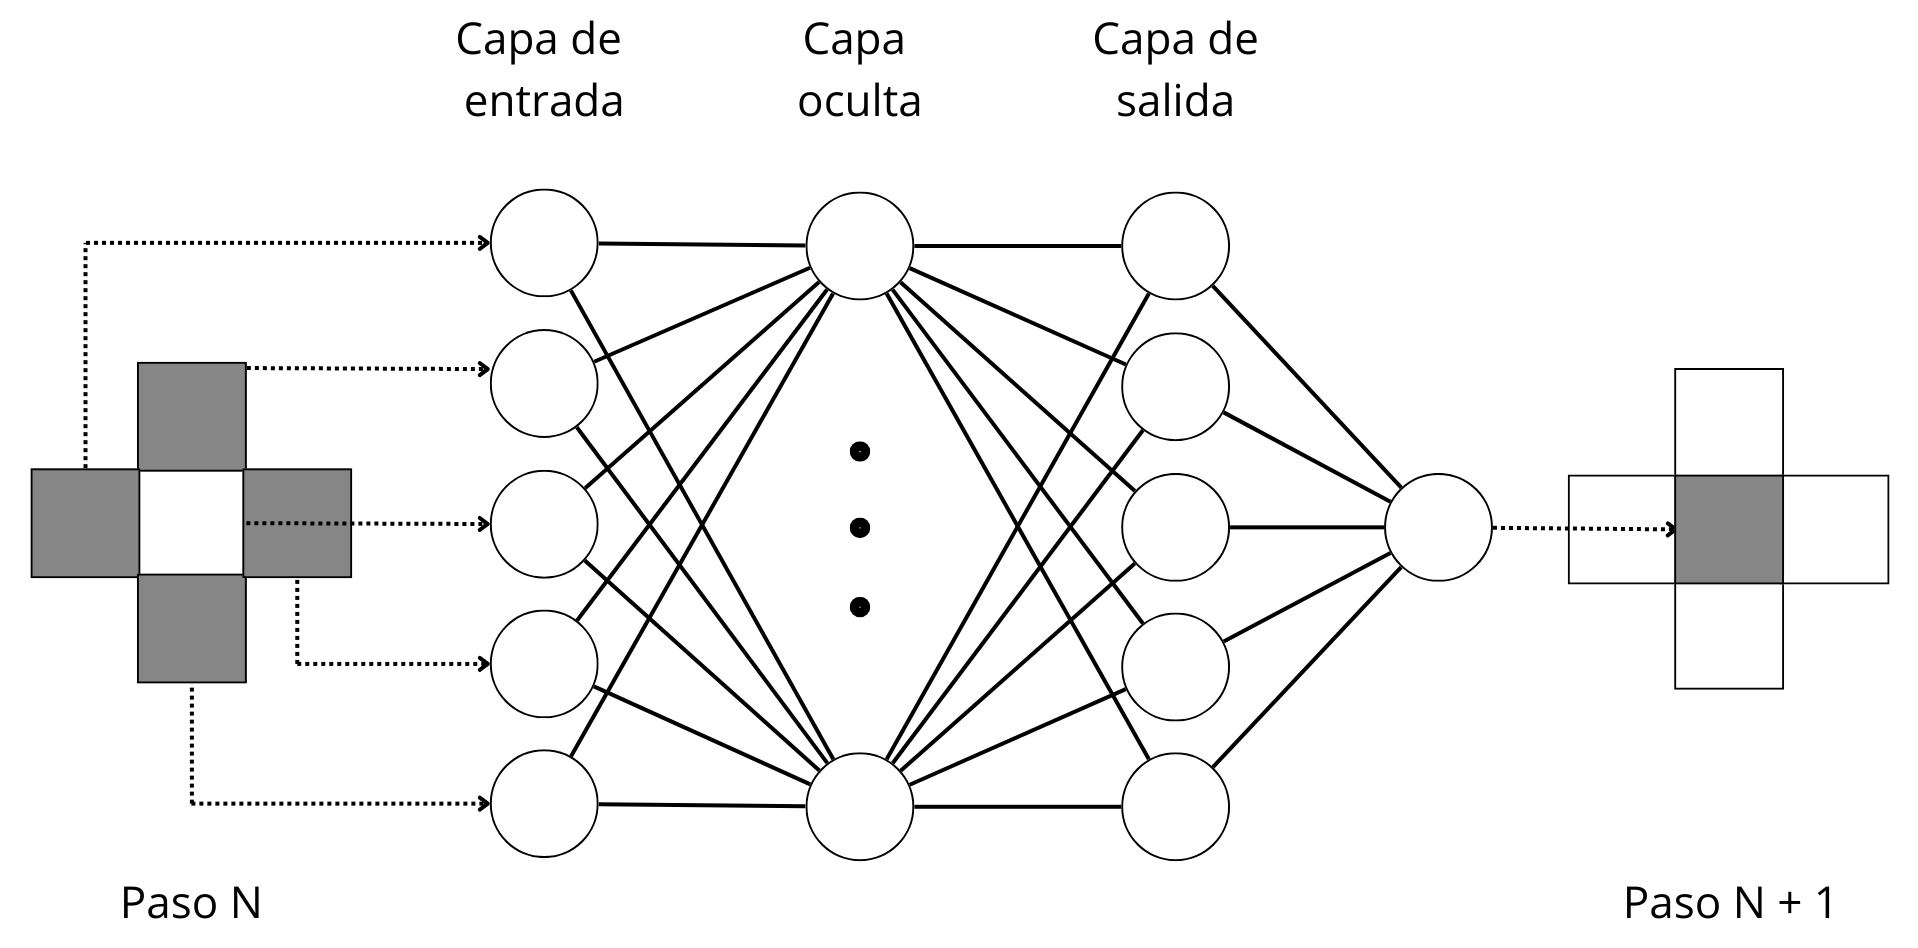
\includegraphics[width=\linewidth]{nca.png}
	\caption{Autómata celular neuronal con vecindad de von Neumann. Los estados de la vecindad en el paso $t$ son la entrada del perceptrón multicapa, cuya salida es el nuevo estado de la célula central en el paso $t+1$.}
	\label{fig:nca}
\end{figure}

En este trabajo, $F_\theta$ es un perceptrón multicapa. Su entrada son los estados de la vecindad, ya sea como números (entrada lineal) o con codificación \onehot{}, en la que cada estado se representa con un vector binario que tiene un solo 1. Esta codificación evita que la red suponga una relación de orden lineal entre estados que no la tienen \cite{MenchacaMendez2022}, por ejemplo, sin ella asume que el estado 2 esté más cerca del 3 que del 9. La capa de salida tiene una neurona por estado y el nuevo estado es el de mayor valor. Para describir la red se usa la notación \red{$L$:$n$:$\varphi$}{$k$:$\psi$}: $L$ capas ocultas de $n$ neuronas con activación $\varphi$ y una capa de salida de $k$ neuronas con activación $\psi$. Por ejemplo, \red{1:4:ReLU}{2:Linear} tiene una capa oculta de 4 neuronas ReLU y dos neuronas de salida lineales.

Como la red es determinista, define una regla local en el sentido de la ecuación~\eqref{eq:regla_local}: basta evaluarla sobre todos los patrones posibles de la vecindad para obtener su vector de regla y compararlo con el de la regla original.

\subsection{Entrenamiento}

Cada célula, en cada paso de la evolución, es una muestra de entrenamiento: la entrada son los estados de su vecindad y la salida esperada es su estado en el paso siguiente. Así, una evolución de $T$ pasos en un espacio de $H \times W$ células aporta $(T-1)\,H\,W$ muestras. Los vecinos que caen fuera del espacio se tratan con frontera periódica o abierta.

La red se entrena con la entropía cruzada como función de pérdida y el optimizador Adam \cite{kingma2015_adam}. La tasa de aprendizaje puede mantenerse constante, reducirse de forma exponencial hasta un valor mínimo o reducirse a la mitad cada vez que la pérdida deja de mejorar durante 20 épocas (reducción por \textit{plateau}). El entrenamiento termina al llegar al número máximo de épocas o cuando la pérdida es menor que la \textit{pérdida objetivo}, que fija qué tan exacta debe ser la regla aprendida.

\subsection{Métricas de evaluación}

Para los sistemas con regla conocida se usan la pérdida, la exactitud de un paso (fracción de células cuyo siguiente estado se predice correctamente) y, en el juego de la vida, la distancia Manhattan entre el vector de la regla original y el de la aprendida.

En los sistemas reales no existe una regla de referencia, por lo que cada red se compara con la predicción sin cambio, que supone que el siguiente paso es igual al actual. Como de un paso a otro cambian pocas células, esta predicción es difícil de superar, pero nunca reproduce la dinámica. Los errores se reportan de forma relativa,
\begin{equation}
	\varepsilon = 100\,\% \cdot \frac{E_{\text{red}}}{E_{\text{sin cambio}}},
	\label{eq:error_relativo}
\end{equation}
de modo que un valor menor que 100\,\% indica que la red mejora a la predicción sin cambio. Además del error de un paso se mide la simulación libre, en la que la red parte de la primera imagen real y evoluciona sola con sus propias predicciones. En FLAME~3 y SEVIR se mide qué tanto se parecen el área quemada o el área con tormenta de la simulación libre a las reales (100\,\% si son idénticas). En \textit{Physarum polycephalum} se usa la coincidencia del plasmodio con
\begin{equation}
	C_t = \frac{|R_t \cap S_t|}{|R_t \cup S_t|} \cdot \frac{\min(|R_t|, |S_t|)}{\max(|R_t|, |S_t|)},
	\label{eq:coincidencia}
\end{equation}
donde $R_t$ y $S_t$ son los conjuntos de células con plasmodio en el paso $t$ de la evolución real y de la simulada. El primer factor mide si el plasmodio está en el mismo lugar y el segundo si hay la misma cantidad; $C_t = 1$ si la simulación es idéntica a la real.

\subsection{Procedimiento experimental}

Los experimentos se dividen en dos series. En la primera, que responde a las preguntas P1 a P3, se entrena el autómata celular neuronal con evoluciones de reglas conocidas (el juego de la vida, la pila de arena y la hormiga de Langton): como la regla original existe, la vecindad correcta determina la transición y la regla aprendida puede compararse con la original. Cada sistema agrega una dificultad: el desbalance de patrones y la vecindad desconocida, un número mayor de estados y la escasez de información. En la segunda serie, que responde a P4, la configuración obtenida se aplica a sistemas reales sin regla conocida y con distinto grado de apertura: la propagación de un incendio (FLAME~3), el movimiento de tormentas (SEVIR) y el crecimiento de moho en una caja de Petri (\textit{Physarum polycephalum}), cada uno con un preprocesamiento propio. La tabla~\ref{tab:experimentos} resume la configuración final de cada experimento. Salvo que se indique otra cosa, se usa una tasa de aprendizaje inicial de 0.001, lotes de 4,096 u 8,192 muestras y la semilla aleatoria 42.

\begin{table*}[!tp]
	\centering
	\small
	\begin{tabularx}{\textwidth}{@{}l c >{\raggedright\arraybackslash}p{2.5cm} >{\raggedright\arraybackslash}X >{\raggedright\arraybackslash}p{4.3cm}@{}}
		\toprule
		\textbf{Sistema} & \textbf{Estados} & \textbf{Vecindad} & \textbf{Datos de entrenamiento} & \textbf{Red seleccionada} \\
		\midrule
		Juego de la vida & 2 & Moore, $3\times3$ (9) & 100 evoluciones aleatorias de B3/S23 en $100\times100$ por 100 pasos & \red{1:4:ReLU}{2:Linear} \\
		Pila de arena & 17 & von Neumann (5) & 2 evoluciones de $25\times25$ durante 2,000 pasos, con 1 y 4 generadoras & \red{2:64:ReLU}{17:Linear}, \onehot{} \\
		Hormiga de Langton & $5n$ (10--50) & Rombo de radio 2 (13) & 2 hormigas en $30\times30$ durante 10,000 pasos, de 2 a 10 colores & \red{4:64:ReLU}{$5n$:Linear}, \onehot{} \\
		FLAME~3 & 18 & $9\times9$ (81) & 1 de 2 secuencias térmicas (116 y 66 imágenes) de $100\times100$ & \red{2:32:ReLU}{18:Linear}, \onehot{}, paso de 30 s \\
		SEVIR & 7 & $11\times11$ (121) & 400 tormentas de 2018, 5 transiciones cada una, $96\times96$ & \red{16:64:ReLU}{7:Linear}, entrada lineal \\
		\textit{Physarum} & 24 & 97 vecinos & 20 cajas de Petri de $160\times160$ células & \red{16:128:ReLU}{24:Linear}, \onehot{} \\
		\bottomrule
	\end{tabularx}
	
	\caption{Resumen de los seis experimentos y de la red seleccionada en cada uno.}
	\label{tab:experimentos}
\end{table*}
